%----------------------------------------------------------------
%
%  File    :  vpn_prelim.tex
%
%  Author  :  Keith Andrews, IICM, TU Graz, Austria
% 
%  Created :  22 Feb 96
% 
%  Changed :  19 Feb 2004
% 
%----------------------------------------------------------------

\chapter{Preliminaries}

\label{chap:Preliminaries}

\section{Mealy Machines}
% TODO: Expand, add grafic or listing, see other papers for inspiration
Mealy machines are finite state machines where each output transition is defined by the current state and an input. More formally, a Mealy machine is defined as a 6-tuple $M = \{S, S_0, \Sigma, \Lambda, T, G\}$, where $S$ is a finite set of states, $S_0 \in S$ is the initial state, $\Sigma$ is a finite set called the input alphabet, $\Lambda$ is a finite set called the output alphabet, $T$ is the transition function $G: S \times \Sigma \rightarrow \Lambda$ which maps a state and an element of the input alphabet to another state in $S$ and $G$ is the output function $T: S \times \Sigma \rightarrow S$ which maps a state-input alphabet pair to an element of the output alphabet $\Lambda$. We use Mealy machines to model the state of learned IPsec implementations.

\section{Automata Learning}

% TODO: More on automata learning, in particular cover L* in detail. Consider what is repeated here from Related chapter.
Automata learning refers to methods of learning the state model, or automaton, of a system through an algorithm or process. We differentiate between active and passive automata learning. In passive automata learning (PAL), models are learned based on a given data set describing the behavior of the SUL, e.g. log files. In contrast, in active automata learning (AAL) the SUL is queried directly. In this paper, we will focus on AAL and will, moving on, be referring to it as automata learning or AAL interchangeably. 

One of the most influential AAL algorithms was introduced in 1987 through a paper by Dana Angluin, titled ``Learning regular sets from queries and counterexamples''~\parencite{ANGLUIN198787}. In this seminal paper, Angluin introduced the $L^*$ algorithm, variants of which are still used for learning deterministic automata to this day, for example by the AAL python library \textsc{AALpy} \parencite{muvskardin2022aalpy}. While the original $L^*$ algorithm was designed to learn deterministic finite automata (DFA), the algorithm can be extended to learn Mealy machines \parencite{Niese2003AnIA}. While many modern implementations, including \textsc{AALpy} use improved versions of $L^*$, fundamentally they still resemble the original algorithm by Angluin. The base $L^*$ algorithm is briefly explained below. TODO: does AALpy version use homing sequences? --> Rivest1993Inference

Another popular algorithm in the field of AAL is the $KV$ algorithm by Kearn's and Vazirani \parencite{KV1994}. Published later than $L^*$, it boasts a more compact method of representing learned data called a classification tree. This, on average, leads to the $KV$ algorithm requiring less membership queries than $L^*$ to learn a system. Especially for learning internet protocols and other systems where communication with the SUL can be very time consuming, this can result in a significant performance increase.

% TODO: expand greatly, go into more detail here
\subsection{L\textsuperscript{*}}
$L^*$ uses a Minimally Adequate Teacher (MAT) model in which a learner queries a teacher in order to learn an unknown regular language $L$. Queries are built using a fixed input alphabet $\Sigma$ where $L \subseteq \Sigma^*$ must hold. The teacher must respond to two types of queries posed by the learner, namely membership and equivalence queries. Membership queries consist of a word $s \in \Sigma^*$ and must be answered with either ``yes'' if $s \in L$, or ``no'' if not. In other words, membership queries are used to check if a given word is part of the language being learned. Equivalence queries on the other hand, consist of a regular language $L_{prop}$, proposed by the learner. The teacher must answer with  ``yes'' if $L_{prop} \equiv L$, or returns a counterexample $c$ proving the two languages are different, so $c \in L(S) \iff c \notin L$. In other words, equivalence queries are used to verify if the learner has successfully learned the target language $L$ or if not, return a counterexample detailing the differences. The results of the membership queries are stored in an observation table $O = (S,E,T)$, where $S$ is a prefix-closed set of strings representing candidates for states of $L_{prop}$, $E$ a suffix-closed set of strings used to distinguish between candidates and $T$ a transition function $(S \cup S \cdot \Sigma) \cdot E \rightarrow {0,1}$. Essentially, if visualized as a 2D array where the rows are labeled with elements in $(S \cup S \cdot \Sigma)$ and columns with elements in $E$, the entries in the table are ones, if the word created by appending the row-label to the column-label is accepted by $L$ and zeros if not. 
The goal of $L^*$ is to learn a DFA acceptor for $L$ using the observation table. S-labeled rows correspond to states in the acceptor under construction. E-labeled columns represent individual membership query results. For the observation table to be transformable into a DFA acceptor, it must first be closed and consistent.


\begin{lstlisting}[mathescape=true, float=ht, caption=$L^*$ algorithm, label=lst:lstar]
	$\mathbf{Initialization}$: 
	Set observation table $O = (S,E,T)$ with $S,E = \{\epsilon\}$.
	$populate(O)$.
	
	$\mathbf{repeat}$:
		$\mathbf{while}$ $O$ is not closed or not consistent $\mathbf{do}$
			$\mathbf{if}$ $O$ is not closed $\mathbf{then}$
				choose $s_1 \in S, \sigma \in \Sigma$ such that
				$row(s_1 \cdot \sigma) \neq row(s) \; \forall s \in S$
				add $s_1 \cdot \sigma$ to $S$
				$populate(O)$
			$\mathbf{end}$
			$\mathbf{if}$ $O$ is not consistent $\mathbf{then}$
				choose $s_1, s_2 \in S, \sigma \in \Sigma$ and $e \in E$ such that
				$row(s_1) = row(s_2)$ and $T(s_1 \cdot \sigma \cdot e) \neq T(s_2 \cdot \sigma \cdot e)$
				add $\sigma \cdot e$ to $E$
				$populate(O)$
			$\mathbf{end}$		
		$\mathbf{end}$
		Construct $L_{prop}$ from $O$ and perform an equivalence query.	
		$\mathbf{if}$ query returns a counterexample $c$ $\mathbf{then}$
			add all prefixes of $c$ to $S$
			$populate(O)$
		$\mathbf{end}$
	$\mathbf{until}$ teacher replies "yes" to equivalence query $L_{prop} \equiv L$
	$\mathbf{return}$ $L_{prop}$
		
\end{lstlisting}

Closed is defined as for all $t \in S \cdot \Sigma$ there exists an $s \in S$ so that $row(t) = row(s)$. In other words, that no new information is gained by expanding the $S$-set by any word in $\Sigma$. If an observation is not closed, it is fixed by adding $t$ to $S$ and updating the table rows through more membership queries. 
Consistent means, that $\forall s_1, s_2 \,|\, row(s_1) = row(s_2) \implies \forall \sigma \in \Sigma \,|\, row(s_1 \cdot \sigma) = row(s_2 \cdot \sigma)$, or in other words, appending the same word to identical states should not result in different outcomes. If an observation table is inconsistent, it is made consistent again by adding another column to the table with the offending $\sigma$ as its label and again updating the table rows through more membership queries. 

Listing~\ref{lst:lstar} shows the workings of the basic $L^*$ algorithm by Angluin. The function $populate(O)$ extends $T$ to $(S \cup S \cdot \Sigma) \cdot E$ by asking membership queries for all table entries still missing membership information. At the start of the algorithm, the observation table is initialized with $S = E = \{\epsilon\}$. Next, until a equivalence query succeeds, the observation table is repeatedly brought to a closed and consistent state by expanding the $S$ and $E$ sets respectively. Once both closed and consistent, $L_{prop}$ is constructed from $O$ and used in an equivalence query. If the equivalence query returns ``yes", the algorithm terminates, returning the learned DFA. If not, the returned counterexample is used to update the observation table and the algorithm loops back to line 5. 


\subsection{KV}
Another notable AAL algorithm is the KV algorithm published in 1994 by Kearns and Vazirani \cite{KV1994}. It is designed to work in the same learner-teacher framework as $L^*$, but was designed to minimize the amount of membership queries needed to learn a finite automaton $M$. The KV algorithm does this by organizing learned information in an ordered binary tree called a classification tree $C_T$ as opposed to the table structure utilized by $L^*$. Intuitively, $L^*$ must perform membership queries for every entry in the observation table to differentiate between possible states, whereas $KV$ requires only a subset to distinguish them. 

In the $KV$ algorithm, learned data is stored in two sets called the access strings set $S$ and the distinguishing strings set $D$. Every string $s \in S$ represents a distinct and unique state of the automaton $M$. In other words, any $s$ when applied starting in the initial state of $M$ leads to a unique state $M[s]$. The distinguishing strings set is defined as the set of strings $d \in D$ where for each pair $s,s' \in S, s \neq s'$ there exists a $d \in D$ such that either $M[s \cdot d]$ or $M[s' \cdot d]$ is an accepting state. $D$ is used to ensure that their are no ambiguous states. The sets $S,D$ are organized in a binary tree called the classification tree $C_T$ where parent nodes are strings from $D$ and the leaf nodes are strings from $S$. The root node is set to the empty string $\lambda$. For each node of the tree, starting from the root node, each right subtree contains access strings to accepting states while left subtrees contain access strings to rejecting states of $M$.
Given a new string $s'$, we simply start at the root nodes, then sift down the tree by executing a membership query for $s' \cdot \lambda_1$ and depending on if the query returns ``yes" or ``no" continuing with the left or right subtree until we reach a leaf node labeled with $s$. If $s' = s$ then the states are equivalent, otherwise the classification tree is updated to include another leaf node representing the newly learned distinct state $s'$. The main learning loop of the $KV$ algorithm is shown in more detail in Listing~\ref{lst:kv}. Following the initialization of the classification table, new states learned from counterexamples are repeatedly added until an equivalence query is successful. The $Update(C_T,c)$ function adds a new leaf to the $C_T$ based on a counterexample $c$ returned from an equivalence query.

\begin{lstlisting}[mathescape=true, float=ht, caption=$KV$ algorithm, label=lst:kv]
	$\mathbf{Initialization}$: 
		Set root node of $C_T$ to $\epsilon$. 
		Perform membership query on $\epsilon$ to determine if the initial state is accepting or not.
		Construct hypothesis automaton $\hat M$ consisting of only the initial state, with self-transitions for all other transitions.
		Add two access strings $\epsilon$ and the counterexample string $c$.
	
	$\mathbf{repeat}$:
		Construct hypothesis automaton $\hat M$ from $C_T$.
		Equivalence query($\hat M$)
		$\mathbf{if}$: query returns "yes" $\mathbf{then}$
			$\mathbf{return}$ $\hat M$
		$\mathbf{end}$
		
		$Update(C_T,c)$
	$\mathbf{end}$
	
\end{lstlisting}


\section{Fuzzing}
% TODO: leave till we actually start this / could write the basics now --> show how model-based fuzzing can worl

\section{IPsec}
% TODO: More on VPNs in general

Virtual Private Networks (VPN) are used to extend and or connect private networks across an insecure channel (usually the public internet). They can be used e.g. to gain additional privacy from prying eyes such as Internet Server Providers, access to region-locked online content or secure remote access to company networks. Many different VPN protocols exit, including PPTP, OpenVPN and Wireguard. IPsec or IP Security, is a VPN layer 3 protocol used to securely communicate over an insecure channel. It is based on three sub-protocols, the Internet Key Exchange (IKE) protocol, the Authentication Header (AH) protocol and the Encapsulating Security Payload (ESP) protocol. IKE is mainly used to handle authentication and to securely exchange as well as manage keys. Following a successful IKE round, either AH or ESP is used to send packets securely between parties. The main difference between AH and ESP is that AH only ensures the integrity and authenticity of messages while ESP also ensures their confidentiality through encryption.

\begin{figure}[H]
\begin{centering}
	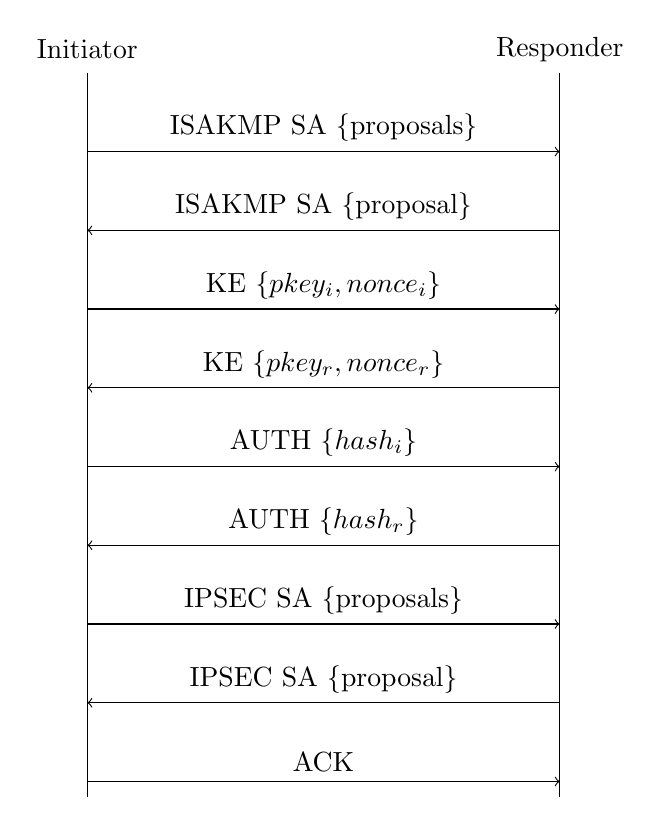
\begin{tikzpicture}[scale=1]
		\draw (-3,0) -- (-3,-9.2) (3,0) -- (3,-9.2);
		\node at (-3,.3) {Initiator};
		\node at (3,.3) {Responder};
		\draw[->] (-3,-1) -- node[midway,above] {ISAKMP SA \{proposals\}} (3,-1);
		\draw[<-] (-3,-2) -- node[midway,above] {ISAKMP SA \{proposal\}} (3,-2);
		\draw[->] (-3,-3) -- node[midway,above] {KE $\{pkey_i, nonce_i\}$} (3,-3);
		\draw[<-] (-3,-4) -- node[midway,above] {KE $\{pkey_r, nonce_r\}$} (3,-4);
		\draw[->] (-3,-5) -- node[midway,above] {AUTH $\{hash_i\}$} (3,-5);
		\draw[<-] (-3,-6) -- node[midway,above] {AUTH $\{hash_r\}$} (3,-6);
		\draw[->] (-3,-7) -- node[midway,above] {IPSEC SA \{proposals\}} (3,-7);
		\draw[<-] (-3,-8) -- node[midway,above] {IPSEC SA \{proposal\}} (3,-8);
		\draw[->] (-3,-9) -- node[midway,above] {ACK} (3,-9);
	\end{tikzpicture}
	\caption{IKEv1 between two parties}
	\label{fig:IKEv1}
\end{centering}
\end{figure}

The IKEv1 protocol works in two main phases, both relying on the Internet Security Association and Key Management Protocol (ISAKMP). Additionally, phase one can be configured to proceed in either Main Mode or Aggressive Mode. A typical exchange between two parties, an initiator and a responder, using Main Mode for phase one, can be seen in Figure \ref{fig:IKEv1}. In phase one (Main Mode), the initiator begins by sending a Security Association (SA) to the responder. A SA essentially details important security attributes required for a connection such as the encryption algorithm and key-size to use, as well as the authentication method and the used hashing algorithm. These options are bundled in containers called proposals, with each proposal describing a possible security configuration. While the initiator can send multiple proposals to give the responder more options to choose from, the responder must answer with only one proposal, provided both parties can agree upon one of the suggested proposals. This initial communication is denoted as \emph{ISAKMP SA} in Figure~\ref{fig:IKEv1}. Subsequently, the two parties perform a Diffie-Hellman key exchange, denoted as \emph{KE}, and send each other nonces used to generate a shared secret key \emph{SKEYID} as detailed in Listing~\ref{lst:keying}. PSK refers to the pre-shared key, Ni/Nr to the initiator/responder nonce and CKY-I/CKY-R to the initiator/responder identifier cookie. Note that IKEv1 allows using various different authentication modes aside from PSK, including public key encryption and digital signatures. \emph{SKEYID} is used as a seed key for all further session keys \emph{SKEYID\_d}, \emph{SKEYID\_a}, \emph{SKEYID\_e}, with $g^{xy}$ referring to the previously calculated shared Diffie-Hellman secret and prf to a pseudo-random function (in our case, HMAC). Following a successful key exchange, all further messages of phase one and two are encrypted using a key derived from \emph{SKEYID\_e} and \emph{SKEYID\_a} for authentication. Finally, in the last section of phase one \emph{AUTH}, both parties exchange and verify hashes to confirm the key generation was successful. Once verification succeeds, a secure channel is created and used for phase two communication. If phase one uses Aggressive Mode, then only three packets are needed to reach phase two. While quicker, the downside of Aggressive Mode is that the communication of the hashed authentication material happens without encryption. This means, that using short pre-shared keys in combination with Aggressive Mode is inherently insecure, as the unencrypted hashes are vulnerable to brute-force attacks provided a short key-size~\footnote{https://nvd.nist.gov/vuln/detail/CVE-2018-5389}. The shorter phase two (Quick Mode) begins with another SA exchange, labeled with \emph{IPSEC SA} in Figure~\ref{fig:IKEv1}. This time, however, the SA describes the security parameters of the ensuing ESP/AH communication and the data is sent authenticated and encrypted using the cryptographic material calculated in phase one. This is followed by a single acknowledge message, \emph{ACK}, from the initiator to confirm the agreed upon proposal. After the acknowledgment, all further communication is done via ESP/AH packets, using \emph{SKEYID\_d} as keying material.

\begin{lstlisting}[float=ht, caption=IKE Keying, label=lst:keying]
	# For pre-shared keys: 
	SKEYID = prf(PSK, Ni_b | Nr_b)
	
	# to encrypt non-ISAKMP messages (ESP)
	SKEYID_d = prf(SKEYID, g^xy | CKY-I | CKY-R | 0)
	
	# to authenticate ISAKMP messages
	SKEYID_a = prf(SKEYID, SKEYID_d | g^xy | CKY-I | CKY-R | 1)
	
	# for further encryption of ISAKMP messages in phase two
	SKEYID_e = prf(SKEYID, SKEYID_a | g^xy | CKY-I | CKY-R | 2)
\end{lstlisting}

In addition to the packets shown in Figure~\ref{fig:IKEv1}, IKEv1 also specifies and uses so called ISAKMP Informational Exchanges. Informational exchanges in IKEv1 are used to send ISAKMP Notify or ISAKMP Delete payloads. Following the key exchange in phase one, all Informational Exchanges are sent encrypted and authenticated. Prior, they are sent in plain. ISAKMP Notify payloads are used to transmit various error and success codes, as well as for keep-alive messages. ISAKMP Delete is used to inform the other communication partner, that a SA has been deleted locally and request that they do the same, effectively closing a connection. 

Compared to other protocols, IPsec offers a high degree of customizability, allowing it to be fitted for many use cases. However, in a cryptographic evaluation of the protocol, Ferguson and Schneier \textcite{ferguson1999cryptographic} criticize the complexity arising from the high degree of customizability as the biggest weakness of IPsec. To address its main criticism, IPsec-IKEv2 was introduced in RFC 7296 to replace IKEv1 \parencite{kaufman2014internet}. Nevertheless, IPsec-IKEv1 is still in wide-spread use to this day, with the largest router producer in Germany, AVM, still only supporting IKEv1 in their routers \parencite{avm2022}. We use IPsec-IKEv1 with Main Mode and ESP in this paper and focus on the IKE protocol as it is the most interesting from an AAL and security standpoint. % this part could maybe be moved to the introduction, not sure
